% YZM5110 Research Project -- presentation slides
% Build:  python scripts/make_report_tables.py && cd slides && tectonic slides.tex
% All measured numbers are macros from ../report/generated/numbers.tex (written from results/ by a script).
% Published numbers are typed by hand and cited on the slide.
\documentclass[aspectratio=169,11pt]{beamer}
\usepackage[T1]{fontenc}
\usepackage{lmodern}
\usepackage{booktabs,amsmath,adjustbox,array}
\usepackage{xcolor}
% generated by scripts/make_report_tables.py -- do not edit
\newcommand{\nQueries}{451}
\newcommand{\nPages}{500}
\newcommand{\nDup}{22}
\newcommand{\pubCard}{0.585}
\newcommand{\pubPaper}{0.544}
\newcommand{\fullB}{0.575}
\newcommand{\fullA}{0.391}
\newcommand{\fullBGE}{0.249}
\newcommand{\gapCardPts}{$-$0.94}
\newcommand{\pubBMtwentyfive}{0.368}
\newcommand{\pubBGE}{0.257}
\newcommand{\fullBnodup}{0.601}
\newcommand{\nDev}{226}
\newcommand{\devB}{0.580}
\newcommand{\devA}{0.400}
\newcommand{\devBGE}{0.235}
\newcommand{\devCkone}{0.534}
\newcommand{\devDkone}{0.526}
\newcommand{\devCksixty}{0.467}
\newcommand{\devDksixty}{0.422}
\newcommand{\devCw}{0.585}
\newcommand{\devDw}{0.580}
\newcommand{\devCwGainPts}{+0.47}
\newcommand{\nWgrid}{9}
\newcommand{\nKgrid}{10}
\newcommand{\nTest}{225}
\newcommand{\testA}{0.382}
\newcommand{\testACI}{[0.323, 0.441]}
\newcommand{\deltaA}{$-$0.188}
\newcommand{\deltaACI}{[$-$0.237, $-$0.142]}
\newcommand{\pHolmA}{$<$0.001}
\newcommand{\pA}{$<$0.001}
\newcommand{\wtlA}{10/144/71}
\newcommand{\testBGE}{0.262}
\newcommand{\testBGECI}{[0.209, 0.317]}
\newcommand{\deltaBGE}{$-$0.308}
\newcommand{\deltaBGECI}{[$-$0.364, $-$0.252]}
\newcommand{\pHolmBGE}{$<$0.001}
\newcommand{\pBGE}{$<$0.001}
\newcommand{\wtlBGE}{5/122/98}
\newcommand{\testB}{0.570}
\newcommand{\testBCI}{[0.510, 0.627]}
\newcommand{\testC}{0.516}
\newcommand{\testCCI}{[0.457, 0.574]}
\newcommand{\deltaC}{$-$0.054}
\newcommand{\deltaCCI}{[$-$0.076, $-$0.032]}
\newcommand{\pHolmC}{$<$0.001}
\newcommand{\pC}{$<$0.001}
\newcommand{\wtlC}{9/167/49}
\newcommand{\testD}{0.519}
\newcommand{\testDCI}{[0.460, 0.578]}
\newcommand{\deltaD}{$-$0.051}
\newcommand{\deltaDCI}{[$-$0.072, $-$0.030]}
\newcommand{\pHolmD}{$<$0.001}
\newcommand{\pD}{$<$0.001}
\newcommand{\wtlD}{4/171/50}
\newcommand{\testCw}{0.571}
\newcommand{\testCwCI}{[0.511, 0.629]}
\newcommand{\deltaCw}{+0.001}
\newcommand{\deltaCwCI}{[$-$0.002, +0.005]}
\newcommand{\pHolmCw}{1.000}
\newcommand{\pCw}{0.937}
\newcommand{\wtlCw}{2/220/3}
\newcommand{\testDw}{0.570}
\newcommand{\testDwCI}{[0.510, 0.627]}
\newcommand{\deltaDw}{+0.000}
\newcommand{\deltaDwCI}{[+0.000, +0.000]}
\newcommand{\pHolmDw}{1.000}
\newcommand{\pDw}{1.000}
\newcommand{\wtlDw}{0/225/0}
\newcommand{\deltaCvsD}{$-$0.003}
\newcommand{\deltaCvsDCI}{[$-$0.027, +0.021]}
\newcommand{\pCvsD}{0.844}
\newcommand{\wtlCvsD}{25/174/26}
\newcommand{\pCwvsDw}{0.937}
\newcommand{\nexact}{93}
\newcommand{\typeexactA}{0.617}
\newcommand{\typeexactB}{0.833}
\newcommand{\typeexactC}{0.774}
\newcommand{\typeexactD}{0.771}
\newcommand{\ngeneral}{115}
\newcommand{\typegeneralA}{0.231}
\newcommand{\typegeneralB}{0.391}
\newcommand{\typegeneralC}{0.345}
\newcommand{\typegeneralD}{0.343}
\newcommand{\nvisual}{17}
\newcommand{\typevisualA}{0.118}
\newcommand{\typevisualB}{0.339}
\newcommand{\typevisualC}{0.265}
\newcommand{\typevisualD}{0.331}
\newcommand{\nNoDup}{212}
\newcommand{\noDupB}{0.598}
\newcommand{\noDupC}{0.542}
\newcommand{\noDupDeltaC}{$-$0.056}
\newcommand{\noDupDeltaCw}{+0.001}
\newcommand{\peakGPU}{15.8}
\newcommand{\latB}{51.3}
\newcommand{\latA}{0.12}
\newcommand{\latBGE}{29.0}
\newcommand{\fusionOverhead}{0.13}
\newcommand{\idxB}{111.7}
\newcommand{\sizeB}{126}
\newcommand{\headallAnotB}{3}
\newcommand{\headallBnotA}{50}
\newcommand{\headexactAnotB}{0}
\newcommand{\headexactBnotA}{22}
\newcommand{\headgeneralAnotB}{3}
\newcommand{\headgeneralBnotA}{23}
\newcommand{\headvisualAnotB}{0}
\newcommand{\headvisualBnotA}{5}
\newcommand{\hitB}{147}
\newcommand{\hitA}{100}
\newcommand{\oracle}{150}
\newcommand{\bothMiss}{75}
\newcommand{\oracleNDCG}{0.588}
\newcommand{\oracleGainPts}{+1.8}
\newcommand{\oracleAbetter}{10}
\newcommand{\cWins}{9}
\newcommand{\cLosses}{49}
\newcommand{\cLossBMmissed}{42}
\newcommand{\cwChanged}{5}
\newcommand{\ovAhit}{0.73}
\newcommand{\ovAmiss}{0.18}
\newcommand{\ovZeroN}{75}
\newcommand{\ovZeroA}{0}
\newcommand{\ovZeroB}{23}
\newcommand{\ovOneN}{43}
\newcommand{\ovOneA}{91}
\newcommand{\ovOneB}{95}

\graphicspath{{../results/figures/}}

% ---- look: plain, readable, palette shared with the figures ------------------------------------------
\definecolor{cpBlue}{HTML}{2a78d6}\definecolor{bmOrange}{HTML}{eb6834}\definecolor{bgAqua}{HTML}{1b7a55}
\definecolor{ink}{HTML}{1f1f1d}\definecolor{muted}{HTML}{6b6a66}\definecolor{tagI}{HTML}{8a6d00}\definecolor{tagH}{HTML}{9b3d8a}
\usetheme{default}
\setbeamertemplate{navigation symbols}{}
\setbeamercolor{frametitle}{fg=cpBlue}
\setbeamercolor{title}{fg=cpBlue}
\setbeamercolor{structure}{fg=cpBlue}
\setbeamercolor{normal text}{fg=ink}
\setbeamerfont{frametitle}{series=\bfseries,size=\Large}
\setbeamertemplate{itemize items}{\textbullet}
\setbeamertemplate{footline}{\hfill\textcolor{muted}{\scriptsize\insertframenumber\,/\,\inserttotalframenumber}\hspace{1em}\vspace{0.6em}}
\newcommand{\lbl}[2]{\textsf{\scriptsize\textcolor{#1}{[#2]}}}
\newcommand{\Pub}{\lbl{cpBlue}{Published}}
\newcommand{\Mea}{\lbl{bgAqua}{Measured}}
\newcommand{\Int}{\lbl{tagI}{Interpretation}}
\newcommand{\Hyp}{\lbl{tagH}{Hypothesis}}
\newcommand{\todo}[1]{\textcolor{red}{\textbf{[TODO: #1]}}}

\title{Does a Lexical Signal Still Help a Visual Retriever?}
\subtitle{Reproducing ColPali on ViDoRe DocVQA and testing BM25 fusion}
\author{\todo{First name LAST NAME}}
\institute{YZM5110 Multimodal Learning --- Research Project}
\date{\todo{presentation date}}

\begin{document}

\begin{frame}
\titlepage
\centering\footnotesize\texttt{github.com/ismailucrn/colpali-hybrid-retrieval}
\end{frame}

% ------------------------------------------------------------------------------------------------------
\begin{frame}{Motivation: two ways to search PDF pages}
\begin{columns}[T]
\column{0.48\linewidth}
\textbf{Text pipeline}\\[2pt]
page $\rightarrow$ OCR / layout $\rightarrow$ chunks $\rightarrow$ BM25 or dense embedding\\[4pt]
\small\textcolor{muted}{slow ingestion; loses layout, figures; OCR errors}
\column{0.48\linewidth}
\textbf{ColPali} (Faysse et al.)\\[2pt]
page \emph{image} $\rightarrow$ vision--language model $\rightarrow$ patch vectors; text query $\rightarrow$ token vectors; late interaction\\[4pt]
\small\textcolor{muted}{no OCR at all}
\end{columns}
\vspace{1em}
\begin{itemize}
  \item \Pub{} ColPali beats every text pipeline on ViDoRe (avg nDCG@5 81.3 vs 67.0).
  \item \Pub{} In \emph{text} retrieval, fusing lexical (BM25) and dense rankings is a cheap, well-known gain --- but not unconditional (Bruch et al., TOIS 2024).
  \item \Int{} Neural retrievers are often said to struggle with exact strings (numbers, codes, names) --- exactly what BM25 matches.
\end{itemize}
\end{frame}

% ------------------------------------------------------------------------------------------------------
\begin{frame}{Research question and pre-registered predictions}
\begin{block}{Question}
Does fusing BM25 (over page text) with ColPali improve page retrieval over ColPali alone --- and for which query types? Is a gain due to the \emph{lexical} signal, or to ensembling with any second retriever?
\end{block}
\vspace{0.4em}
Written \textbf{before} any fusion run (git commits \texttt{162441e}, \texttt{55fa350}, \texttt{2dfcf31}):
\begin{itemize}
  \item \textbf{P1} \; C = RRF(BM25, ColPali) $>$ ColPali on test nDCG@5
  \item \textbf{P2} \; gain concentrated on \emph{exact-match} queries, little on visual ones
  \item \textbf{P3} \; C $>$ D = RRF(\emph{dense} text retriever, ColPali) \quad (control)
\end{itemize}
\small\textcolor{muted}{What would weaken it: no gain; gain spread evenly or on visual queries; D $\ge$ C.}
\end{frame}

% ------------------------------------------------------------------------------------------------------
\begin{frame}{How ColPali scores a page}
\begin{columns}[c]
\column{0.55\linewidth}
\begin{itemize}
  \item \Pub{} PaliGemma-3B encodes the page image; every output vector projected to 128-d.
  \item \Mea{} 1031 vectors per page; \sizeB{}\,MB for \nPages{} pages (bf16).
  \item Query: tokens + 5 augmentation tokens.
  \item \textbf{Late interaction (MaxSim)}, from ColBERT:
\end{itemize}
\[
s(q,d)=\sum_{i \in q}\;\max_{j \in d}\;\langle E_q^{(i)},E_d^{(j)}\rangle
\]
\column{0.42\linewidth}
\small
\Int{} Each query token finds the patch where its word is \emph{printed} --- a kind of ``visual lexical matching'' without OCR.\\[6pt]
We use the authors' checkpoint (v1.3), \textbf{inference only}.
\end{columns}
\end{frame}

% ------------------------------------------------------------------------------------------------------
\begin{frame}{Literature: what is known about text + visual fusion}
\small
\begin{tabular}{@{}p{3.2cm}p{9.6cm}@{}}
\toprule
RRF (Cormack 2009) & \Pub{} beats single runs when fusing \emph{many} runs of similar quality; $k{=}60$\\
Bruch et al.\ (TOIS 2024) & \Pub{} default RRF falls \emph{below} the better input on 4/9 datasets\\
DSE (EMNLP 2024) & \Pub{} screenshot + text hybrid: ``minimal improvement''\\
IRPAPERS (2026) & \Pub{} fusion helps (R@1 49 vs 43) --- clean LLM transcriptions, text $\approx$ image\\
Slide study (2025) & \Pub{} RRF[ColPali, text] 81.0 vs ColPali 82.7 nDCG@10\\
ViDoRe V1/V2 & \Pub{} visual retrievers evaluated \emph{against} or \emph{without} text, never combined\\
\bottomrule
\end{tabular}
\vspace{0.8em}
\begin{block}{Gap \Int{}}
Mixed, uncontrolled results: no significance tests, no ``any second retriever'' control, no per-query-type analysis, none on a ViDoRe task with the benchmark's OCR.
\end{block}
\footnotesize\textcolor{muted}{8 papers in the matrix (\texttt{docs/literature\_matrix.md}); gap narrowed after a targeted search on 6 Nov --- stated in the report.}
\end{frame}

% ------------------------------------------------------------------------------------------------------
\begin{frame}{Reproduction: ColPali on ViDoRe DocVQA}
\small Claim tested: the authors' DocVQA nDCG@5. Tolerance fixed before the run: $\pm$2 points.\\[4pt]
\begin{adjustbox}{max width=\linewidth}
\begin{tabular}{lrlrr}
\toprule
System & Published & source & Measured & $\Delta$\\
\midrule
\textbf{ColPali v1.3} & \pubCard & model card & \textbf{\fullB} & \gapCardPts{} pt\\
BM25 (OCR text) & \pubBMtwentyfive & paper Tab.~2 & \fullA & \textcolor{muted}{different OCR}\\
BGE-M3 (OCR text) & \pubBGE & paper Tab.~2 & \fullBGE & \textcolor{muted}{different OCR}\\
\bottomrule
\end{tabular}
\end{adjustbox}
\vspace{0.6em}
\begin{itemize}
  \item \Mea{} \textbf{Reproduced} within tolerance (\nQueries{} queries, \nPages{} pages, official protocol).
  \item Authors' code (\texttt{colpali-engine}), pinned model + data revisions, Colab L4, bf16.
  \item Our evaluator matches MTEB exactly (max $|\Delta|$ = 0); scores re-evaluated on CPU.
  \item Deviation: v1.3 instead of the paper's v1.0 (\pubPaper) --- v1.0 unsupported in current code.
\end{itemize}
\end{frame}

% ------------------------------------------------------------------------------------------------------
\begin{frame}{Experimental design}
\begin{columns}[T]
\column{0.5\linewidth}
\textbf{Systems}\\[2pt]
\small
\begin{tabular}{@{}ll@{}}
A & BM25 on Tesseract OCR text\\
B & ColPali v1.3\\
C & RRF(A, B) \hfill\textcolor{muted}{proposed}\\
D & RRF(BGE-M3, B) \hfill\textcolor{muted}{control}\\
E & $k$ sweep; weighted RRF \hfill\textcolor{muted}{ablation}\\
\end{tabular}\\[6pt]
D reads the \emph{same} OCR text, same corpus, same RRF, same tuning budget.
\column{0.48\linewidth}
\small
\begin{itemize}
  \item Query tags from text only, frozen: exact / general / visual
  \item Split 50/50 stratified: dev \nDev{} / test \nTest{}
  \item $k$ and weights chosen on \textbf{dev}; test run \textbf{once} (script refuses changed settings)
  \item Bootstrap 95\% CIs, paired permutation test, Holm correction
  \item Resource cost: index time/size, latency, memory
\end{itemize}
\end{columns}
\end{frame}

% ------------------------------------------------------------------------------------------------------
\begin{frame}{Dev: fusion is below ColPali at every $k$}
\begin{columns}[c]
\column{0.56\linewidth}
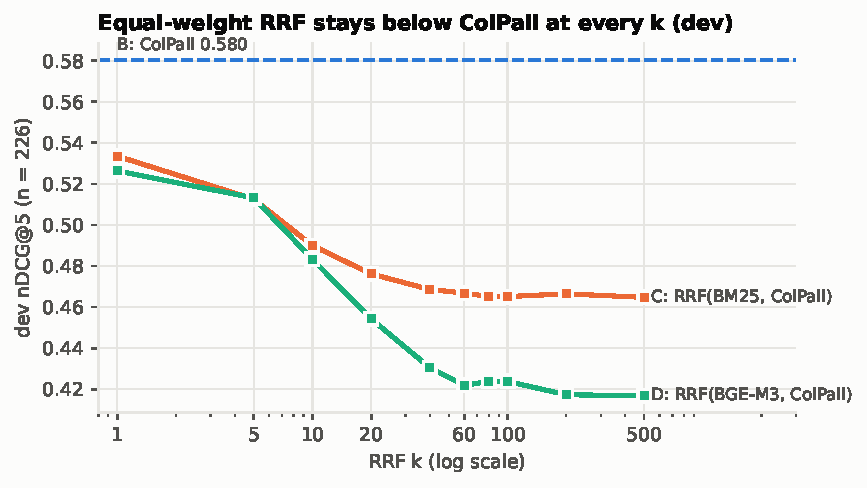
\includegraphics[width=\linewidth]{fig2_dev_k_sweep.pdf}
\column{0.42\linewidth}
\small
\begin{itemize}
  \item \Mea{} ColPali \devB{}; best C \devCkone{}, best D \devDkone{} (both at $k{=}1$)
  \item default $k{=}60$: C \devCksixty{}
  \item Weighted RRF (added after this, labelled \emph{dev-informed}): only $w \ge 0.9$ avoids harm; best C$_w$ \devCwGainPts{} pt on dev
  \item \Int{} the best fusion is the one that changes ColPali least
\end{itemize}
\end{columns}
\end{frame}

% ------------------------------------------------------------------------------------------------------
\begin{frame}{Test (run once): fusion does not help}
\begin{columns}[c]
\column{0.58\linewidth}
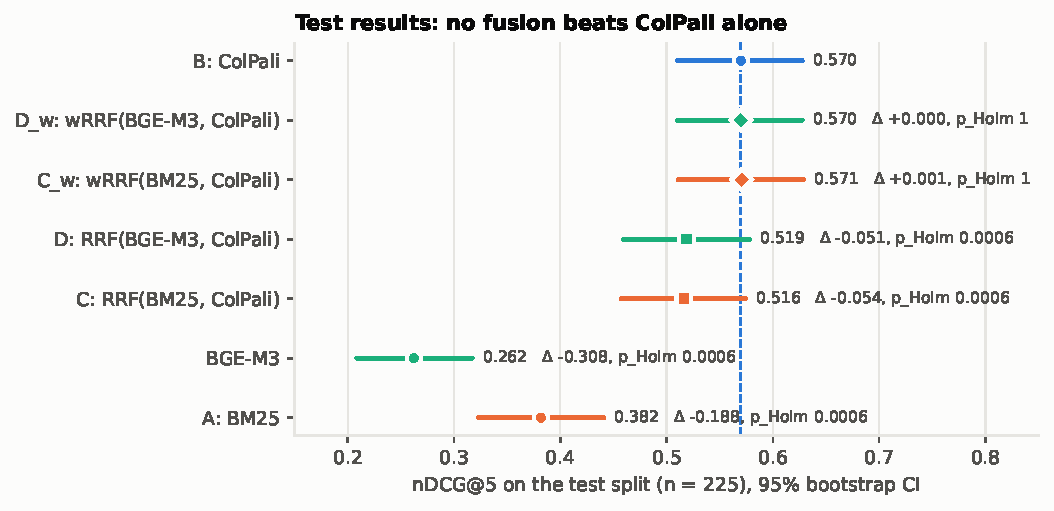
\includegraphics[width=\linewidth]{fig1_test_ndcg5.pdf}
\column{0.40\linewidth}
\small \Mea{} nDCG@5, $n$ = \nTest{}\\[4pt]
ColPali \textbf{\testB{}}\\
C \testC{} \quad $\Delta$ \textbf{\deltaC{}}, $p_\text{Holm}$ \pHolmC{}\\
D \testD{} \quad $\Delta$ \deltaD{}\\
C$_w$ \testCw{} \quad $\Delta$ \deltaCw{}, $p$ \pCw{}\\[6pt]
\begin{itemize}
  \item \textbf{P1 rejected} --- significant harm
  \item \textbf{P3 not supported} --- C$-$D \deltaCvsD{}, $p$ \pCvsD{}
  \item dev gain of C$_w$ was selection noise
\end{itemize}
\end{columns}
\end{frame}

% ------------------------------------------------------------------------------------------------------
\begin{frame}{By query type: the premise of P2 is reversed}
\centering
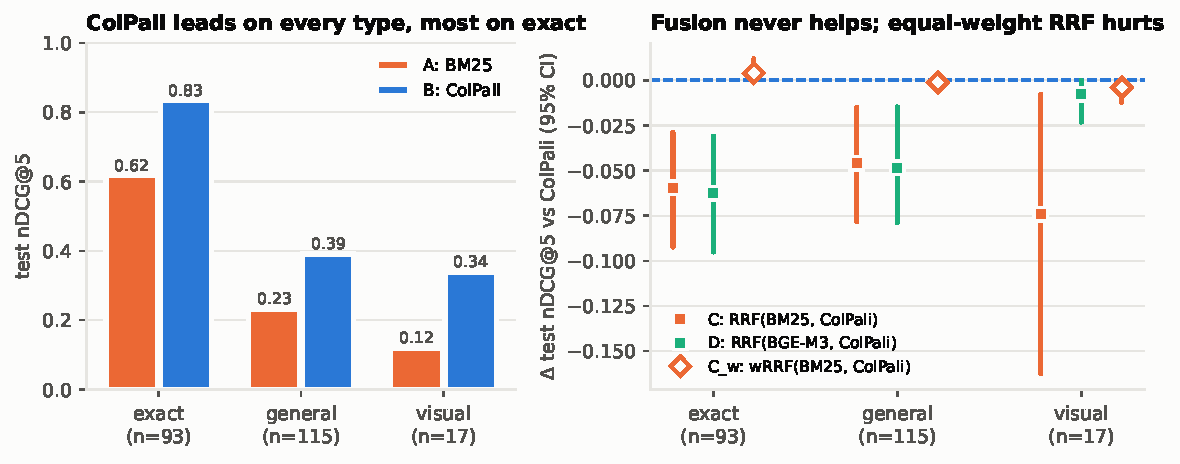
\includegraphics[width=0.78\linewidth]{fig4_test_by_type.pdf}\\[2pt]
\small\raggedright
\Mea{} ColPali is strongest on \emph{exact} queries (\typeexactB{} vs BM25 \typeexactA{}); fusion loses there too (C \typeexactC{}). Visual: $n$ = \nvisual{}, wide CIs. \textbf{P2 not supported.}
\end{frame}

% ------------------------------------------------------------------------------------------------------
\begin{frame}{Why: BM25 finds almost nothing ColPali misses}
\begin{columns}[c]
\column{0.58\linewidth}
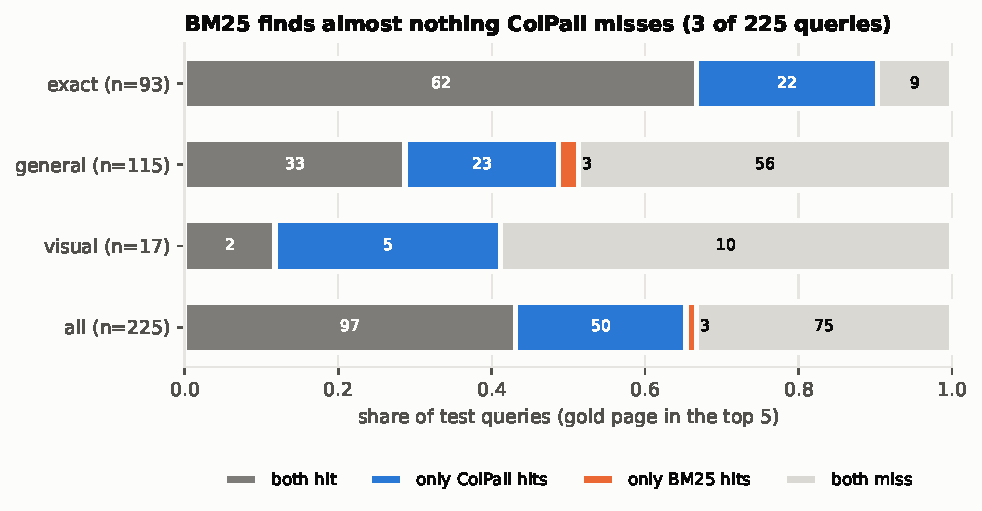
\includegraphics[width=\linewidth]{fig5_headroom.pdf}
\column{0.40\linewidth}
\small \Mea{} gold page in top 5 (test):
\begin{itemize}
  \item BM25 only: \textbf{\headallAnotB{}} queries (0 exact)
  \item ColPali only: \headallBnotA{}
  \item per-query oracle: nDCG@5 \oracleNDCG{} vs \testB{} (\oracleGainPts{} pt)
  \item C's \cLosses{} losses: \cLossBMmissed{} are queries where BM25 had missed
\end{itemize}
\Int{} little to gain, much to lose --- explains P1 and P3
\end{columns}
\end{frame}

% ------------------------------------------------------------------------------------------------------
\begin{frame}{Mechanism: BM25 needs the query's words in the OCR text}
\begin{columns}[c]
\column{0.56\linewidth}
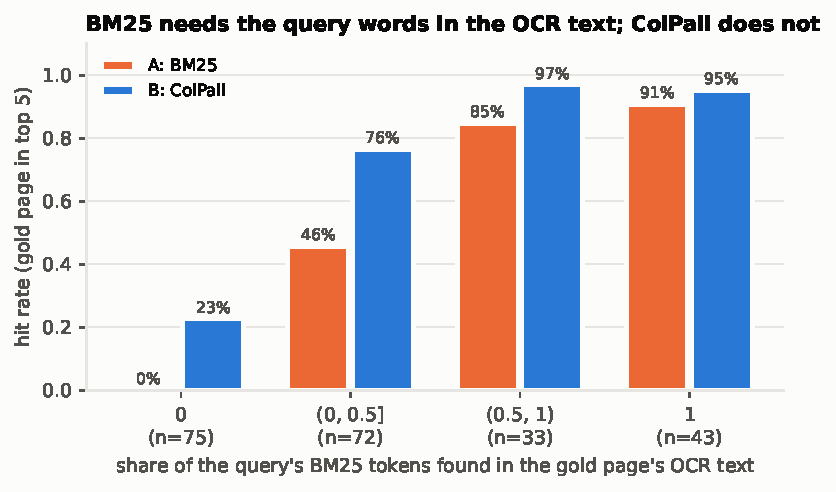
\includegraphics[width=\linewidth]{fig6_overlap.pdf}
\column{0.42\linewidth}
\small \Mea{} overlap = share of query tokens found in the gold page's OCR
\begin{itemize}
  \item zero overlap (\ovZeroN{} q.): BM25 \ovZeroA{}\%, ColPali \ovZeroB{}\%
  \item full overlap (\ovOneN{} q.): BM25 \ovOneA{}\%, ColPali \ovOneB{}\%
\end{itemize}
\Int{} ColPali reads the page image and still matches when OCR or tokenisation lost the words.
\end{columns}
\end{frame}

% ------------------------------------------------------------------------------------------------------
\begin{frame}{Examples (rank of the gold page)}
\small
\begin{tabular}{@{}>{\raggedright\arraybackslash}p{5.6cm}rrrl@{}}
\toprule
query & ColPali & BM25 & C & why\\
\midrule
\multicolumn{5}{@{}l}{\textbf{Unfavourable} --- C worse than ColPali (\cLosses{} of \nTest{})}\\
``What is No.~2-26 of subheading H?'' & 1 & 342 & 3 & ``No'' stopword, ``2-26'' dropped\\
``What is the VO.~NO.?'' & 1 & 137 & 3 & OCR reads ``YO.~NO.''\\
``\dots\ postal stamp at top left?'' & 3 & 252 & 7 & page has \emph{empty} OCR\\
\midrule
\multicolumn{5}{@{}l}{\textbf{Favourable} --- C better than ColPali (\cWins{} of \nTest{})}\\
``What is the name of the laboratory?'' & 14 & 3 & 4 & real lexical rescue\\
``How many bullet points are there?'' & 136 & 2 & 4 & \Int{} probably lucky\\
``Who is from Indiana?'' & 2 & 1 & 1 & typical case: rank 2 $\rightarrow$ 1\\
\bottomrule
\end{tabular}\\[6pt]
\footnotesize\textcolor{muted}{\Mea{} all cases: \texttt{results/failure\_analysis/examples.md}}
\end{frame}

% ------------------------------------------------------------------------------------------------------
\begin{frame}{Post-hoc checks: is it the fusion function, or the tokenizer?}
\small Pre-registered after the main test run (\texttt{cb332b7}); chosen on dev, test evaluated once --- \textbf{exploratory}.\\[6pt]
\begin{columns}[T]
\column{0.48\linewidth}
\textbf{Score-level fusion} (Bruch et al.)\\[2pt]
$\alpha\,\mathrm{mm}(\text{ColPali}) + (1-\alpha)\,\mathrm{mm}(\text{text})$
\begin{itemize}
  \item \Mea{} dev: every $\alpha<1$ below ColPali (best \devBestBelowOneCcc{} vs \devB{})
  \item rule selects $\alpha = 1$ = ColPali alone, for BM25 \emph{and} BGE-M3
  \item \Int{} not specific to rank fusion
\end{itemize}
\column{0.48\linewidth}
\textbf{Code-preserving BM25 tokenizer}\\[2pt]
keeps ``no'' and ``2-26''-style codes
\begin{itemize}
  \item \Mea{} BM25 \testA{} $\rightarrow$ \testAcode{} ($\Delta$ \deltaAcodeA{}, $p$ \pAcodeA{}); exact \typeexactA{} $\rightarrow$ \typeexactAcode{}
  \item but BM25-only hits stay at \headAcodeOnly{}
  \item RRF still hurts: $\Delta$ \deltaCcode{}, $p_\text{Holm}$ \pHolmCcode{}
  \item \Int{} better BM25 only where ColPali is already right
\end{itemize}
\end{columns}
\end{frame}

% ------------------------------------------------------------------------------------------------------
\begin{frame}{Cost: fusion is cheap --- quality is the obstacle}
\centering
{\scriptsize\begin{adjustbox}{max width=\linewidth}
\begin{tabular}{lrrrrr}
\toprule
System & Index time (s) & Index size (MB) & Latency seq.\ (ms) & Latency par.\ (ms) & Fusion (ms) \\
\midrule
A & 0.35 & 0.63 & 0.12 & 0.12 & 0.00 \\
BGE-M3 & 21.10 & 1.95 & 29.04 & 29.04 & 0.00 \\
B & 111.70 & 125.85 & 51.30 & 51.30 & 0.00 \\
C & 112.04 & 126.48 & 51.55 & 51.43 & 0.13 \\
D & 132.79 & 127.81 & 80.47 & 51.43 & 0.13 \\
C$_w$ & 112.04 & 126.48 & 51.56 & 51.44 & 0.14 \\
D$_w$ & 132.79 & 127.81 & 80.47 & 51.43 & 0.13 \\
\bottomrule
\end{tabular}
\end{adjustbox}
\par\smallskip{\footnotesize Medians over single queries. Components were measured on different devices: ColPali on an NVIDIA L4 (bf16, peak GPU memory 15.8~GiB), BGE-M3 on Apple M5 MPS (fp16), BM25 and fusion on the M5 CPU. Sequential = sum of components + fusion; parallel = slowest component + fusion.}
}
\vspace{0.2em}
\raggedright
\small
\begin{itemize}
  \item \Mea{} fusion itself \fusionOverhead{}\,ms/query; BM25 index 0.6\,MB vs ColPali \sizeB{}\,MB
  \item parallel retrieval: latency set by ColPali (\latB{}\,ms on L4)
  \item ColPali peak GPU memory \peakGPU{}\,GiB \Hyp{} full-vocabulary logits --- not investigated
\end{itemize}
\end{frame}

% ------------------------------------------------------------------------------------------------------
\begin{frame}{Limitations}
\begin{itemize}
  \item One task (DocVQA), one OCR (Tesseract), one checkpoint (v1.3)
  \item \Pub{} DocVQA is in ColPali's training data (split not stated) --- favours ColPali vs zero-shot text baselines
  \item Test set: \nTest{} queries, only \nvisual{} visual --- wide CIs, per-type results exploratory
  \item Score-level fusion and tokenizer tested only post-hoc, one design each (min-max; one tokenizer)
  \item Main run keeps the official BM25 preprocessing (drops ``no'', ``2-26'') for comparability
  \item Resource numbers from three devices (L4, M5 MPS, M5 CPU)
  \item Reproduction gap (\gapCardPts{} pt) not traced to a cause
\end{itemize}
\end{frame}

% ------------------------------------------------------------------------------------------------------
\begin{frame}{Conclusions and open questions}
\begin{itemize}
  \item \Mea{} ColPali's DocVQA result reproduces with the authors' code and checkpoint.
  \item \Mea{} Adding BM25 by RRF \textbf{hurts} (\deltaC{} nDCG@5); a dense-text control hurts equally; the best dev-tuned weighting only ties; post-hoc, score-level fusion picks ColPali alone and a better tokenizer adds no headroom.
  \item \Int{} On DocVQA, ColPali already reads the lexical anchors BM25 needs --- better than Tesseract OCR does. Fusion with a much weaker ranking imports its errors.
  \item \Int{} Consistent with when fusion fails in text IR (unequal inputs) and when text + visual fusion helped (clean text, equal strength).
\end{itemize}
\vspace{0.4em}
\textbf{Open} \Hyp{}
\begin{itemize}
  \item Fusion should help once the OCR text itself improves (layout-aware / LLM OCR) or on text-dense corpora --- the tokenizer alone was not enough.
  \item On ViDoRe V2 (less lexical overlap by design), even less.
\end{itemize}
\end{frame}

% ------------------------------------------------------------------------------------------------------
\begin{frame}{Reproducibility and AI use}
\small
\begin{itemize}
  \item Public repo: configs, pinned dependencies and revisions, committed score matrices, every console log, run registry with failed runs
  \item Every number in report and slides is generated from \texttt{results/} by a script
  \item \Mea{} Fresh-clone check (11 Nov): CPU pipeline re-run without torch --- all outputs identical, figures pixel-identical
  \item Pre-registration is checkable in git history (split, control, ablation committed before the test run)
\end{itemize}
\vspace{0.4em}
\textbf{AI use (disclosed, \texttt{docs/ai\_usage.md})}: Claude Code wrote most code, drove Colab, extracted literature details and drafted documents; the author chose task, checkpoint, control and every pre-registration, approved each run, and verified \todo{what you checked}.\\[6pt]
\centering\texttt{github.com/ismailucrn/colpali-hybrid-retrieval} \quad tag \texttt{v1.0-submission}
\end{frame}

% ------------------------------------------------------------------------------------------------------
\appendix
\begin{frame}{Backup: weighted RRF grid on dev}
\centering
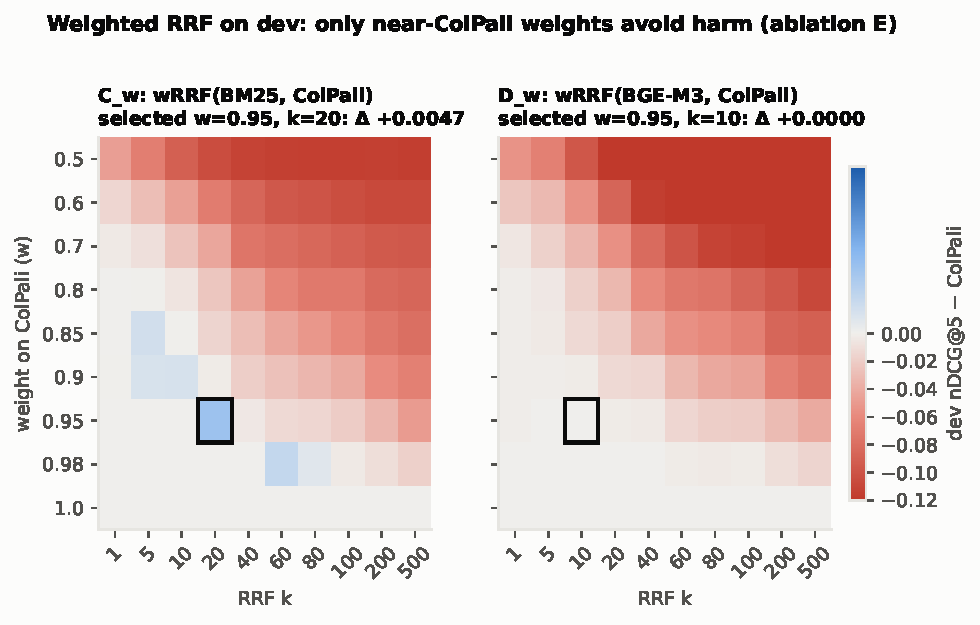
\includegraphics[height=0.72\textheight]{fig3_dev_weighted_rrf.pdf}\\
\small \Mea{} $\Delta$nDCG@5 vs ColPali; only $w \ge 0.9$ (ColPali weight) avoids harm.
\end{frame}

\begin{frame}{Backup: full test table}
\centering
\footnotesize
\begin{adjustbox}{max width=\linewidth}
\begin{tabular}{llllllll}
\toprule
System & Role & nDCG@5 [95\% CI] & R@5 & R@10 & MRR@10 & $\Delta$ vs B [95\% CI] & $p_\mathrm{Holm}$ \\
\midrule
A & text baseline & 0.382 [0.323, 0.441] & 0.444 & 0.498 & 0.369 & $-$0.188 [$-$0.237, $-$0.142] & $<$0.001 \\
BGE-M3 & D's text part & 0.262 [0.209, 0.317] & 0.307 & 0.418 & 0.262 & $-$0.308 [$-$0.364, $-$0.252] & $<$0.001 \\
B & reproduced baseline & 0.570 [0.510, 0.627] & 0.653 & 0.680 & 0.546 & -- & -- \\
C & proposed & 0.516 [0.457, 0.574] & 0.618 & 0.667 & 0.489 & $-$0.054 [$-$0.076, $-$0.032] & $<$0.001 \\
D & control & 0.519 [0.460, 0.578] & 0.609 & 0.667 & 0.496 & $-$0.051 [$-$0.072, $-$0.030] & $<$0.001 \\
C$_w$ & ablation E & 0.571 [0.511, 0.629] & 0.653 & 0.680 & 0.547 & +0.001 [$-$0.002, +0.005] & 1.000 \\
D$_w$ & ablation E & 0.570 [0.510, 0.627] & 0.653 & 0.680 & 0.546 & +0.000 [+0.000, +0.000] & 1.000 \\
\bottomrule
\end{tabular}
\end{adjustbox}
\par\smallskip{\footnotesize Test split, 225 queries, run once with settings frozen on dev. CI: percentile bootstrap over queries (10{,}000 resamples). $p$: two-sided paired sign-flip permutation test (10{,}000), Holm-corrected over the six comparisons with B.}

\vspace{0.5em}
\raggedright
\Mea{} Post-hoc without the \nDup{} duplicated query texts ($n$ = \nNoDup{}): ColPali \noDupB{}, C $\Delta$ \noDupDeltaC{}, C$_w$ $\Delta$ \noDupDeltaCw{} --- same picture.
\end{frame}

\begin{frame}{Backup: by query type with tests}
\centering
\footnotesize
\begin{adjustbox}{max width=\linewidth}
\begin{tabular}{llll}
\toprule
System & exact ($n$=93) & general ($n$=115) & visual ($n$=17) \\
\midrule
A & 0.617 ($-$0.217, $p<0.001$) & 0.231 ($-$0.160, $p<0.001$) & 0.118 ($-$0.221, $p=0.061$) \\
BGE-M3 & 0.458 ($-$0.376, $p<0.001$) & 0.130 ($-$0.261, $p<0.001$) & 0.088 ($-$0.251, $p=0.058$) \\
B & 0.833 & 0.391 & 0.339 \\
C & 0.774 ($-$0.059, $p<0.001$) & 0.345 ($-$0.046, $p=0.006$) & 0.265 ($-$0.074, $p=0.128$) \\
D & 0.771 ($-$0.063, $p<0.001$) & 0.343 ($-$0.048, $p=0.002$) & 0.331 ($-$0.008, $p=1.000$) \\
C$_w$ & 0.837 (+0.004, $p=1.000$) & 0.390 ($-$0.001, $p=0.743$) & 0.335 ($-$0.004, $p=1.000$) \\
D$_w$ & 0.833 (+0.000, $p=1.000$) & 0.391 (+0.000, $p=1.000$) & 0.339 (+0.000, $p=1.000$) \\
\bottomrule
\end{tabular}
\end{adjustbox}
\par\smallskip{\footnotesize Test nDCG@5 by frozen query tag; in brackets $\Delta$ vs B and the uncorrected permutation $p$ (exploratory).}

\end{frame}

\end{document}
